\chapter{Design of Experiments}\label{ch:design-experiments}
\initial{C}hapter: ~\ref{ch:research-methodology} documents the design of the hardware and algorithmic implementations of the system that was used.
Section: ~\ref{sec:op-params} shows some of the results obtained in a configuration step and determining the limitations of the unprocessed data.
To evaluate the performance of the designs, several Test suites were planned which exploited the No Line of Sight (NLOS) issue seen in previous sections.
To provide NLOS, rather than systematically occlude an anchor and tag, a person walked a fixed path (see Figure:~\ref{fig:occlude}) at random speeds whilst the data was being recorded.
This was done as to emulate a more realistic environment that the system would be used in.

For tests that had the tag moving two trajectories were outlined.
Table:~\ref{tb:trajs} shows the waypoints of each of the trajectories.
Trajectory one is a quadrilateral whilst trajectory two is a combination of straight-line segments.
In these tests, the tag was moved along the chosen trajectory whilst NLOS occurred randomly due to a person walking.


\begin{figure}[ht!]
    \centering
    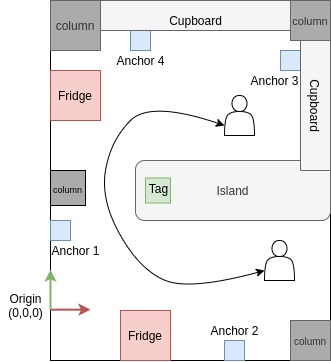
\includegraphics[scale=0.8]{Test_procedure}
    \caption{Path taken by the person to randomly occlude anchors and tag.}
    \label{fig:occlude}
\end{figure}

\begin{table}[ht!]
    \centering
    \begin{tabular}{|c|c|}
        \hline
        & Waypoints $(x,y)$(mm)\\
        \hline
        Trajectory 1 & $\begin{array}{c}
                            (1610, 2080)\\
                            (2111, 2080)\\
                            (1910, 2380)\\
                            (1610, 2580)\\
                            (1610, 2080)
        \end{array}$\\
        \hline
        Trajectory 2 & $\begin{array}{c}
                            (1610, 2080)\\
                            (1710, 2200)\\
                            (1760, 2300)\\
                            (1770, 2500)\\
                            (1840, 2580)\\
                            (1934, 2625)\\
                            (1992, 2595)
        \end{array}$\\
        \hline
    \end{tabular}
    \caption{Trajectories used in the tests for data collection.}
    \label{tb:trajs}
\end{table}
\newpage
\section{Benchmarking and Calibration}\label{sec:benchmarking}
Before testing the system with limitations a benchmark and calibration test was run to record results in an ideal scenario.
This test provided a base that can be used to compare the results of the system operating in non-ideal situations.
Figure: ~\ref{fig:los} shows the results obtained for this benchmarking.
It is seen although the measured position from the tag is slightly noisy, it is well within the $\pm10$cm accuracy quoted by the Pozyx system once the system has started moving and some time has passed.
\begin{figure}[h!]
    \centering
    \begin{subfigure}{0.49\textwidth}
            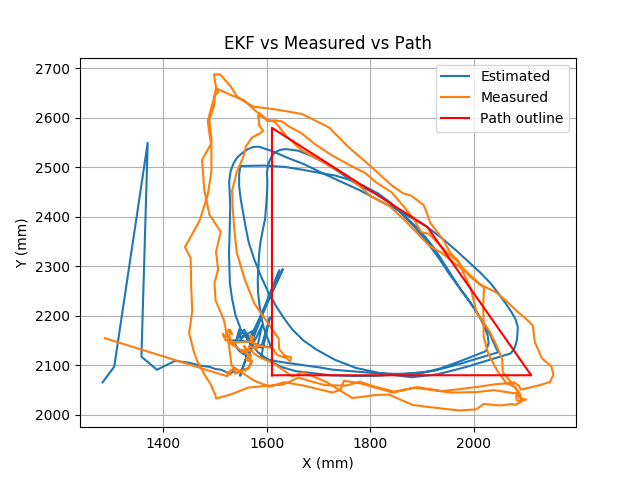
\includegraphics[width=\textwidth]{results/triangle_path_los}
            \caption{Person moving Tag on Trajectory 1.}
    \end{subfigure}
    \begin{subfigure}{0.49\textwidth}
            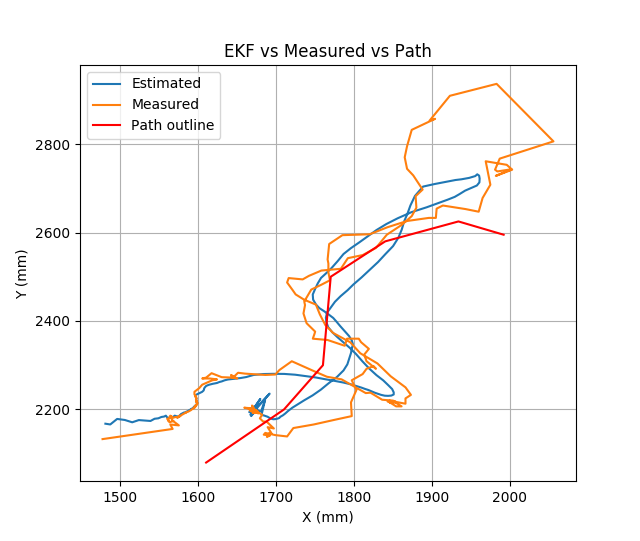
\includegraphics[width=\textwidth]{results/c_path_los}
            \caption{Person moving Tag on Trajectory 2.}
    \end{subfigure}
    \caption{Results for estimation with Line of Sight}
    \label{fig:los}
\end{figure}